\section{Critical Core Radius}

Neutronic viability is an important part of reactor design. The figure of merit
for neutronics is EOL \keff. The reactor must be able to sustain a fission
chain reaction from startup to shutdown on the final day of the 10 year mission.

The criticality requirement is the second of two major criteria for a valid reactor design and an
important constraint in the thermal hydraulic modeling process. As a result,
modeling criticality of various reactor configurations demands its own chapter
in this thesis. Criticality modeling started with depletion modeling, reported
in section \ref{neutronics_sweeps}. The purpose and conclusion of the depletion
modeling was that thermal power and small geometric features were of low
importance when predicting EOL \keff. In addition, higher enrichment will always
be prefferred to lower enriched uranium.

The thermal-hydraulic modeling scheme
reported in section \ref{reactor_mass_model} requires a constraint for the core
radius. A relationship between core radius and fuel fraction for a target
value of \keff was developed using traditional reactor physics tools. In lieu of
full depletion modeling, BOL \keff was modeled and the \keff target adjusted to
ensure sufficient excess reactivity for 10 years of full-power operation.

There were three major components to developing the critical core radius
constraints, determining a value for BOL excess reactivity that would satisfy
EOL \keff > 1, optimizing the reflector radius for each fuel type to minimize
overall mass, and generating the relationship between fuel fraction and the
required core radius to meet the target \keff value. Critical core radius is a
bit of a misnomer, since the target of this analysis was a BOL excess
reactivity.

\subsection{Optimized Reflector Thicknesses}
Reflectors are used in nuclear reactor design to reduce neutron leakage from the
reactor core. Reflectors can reduce required fuel mass by reflecting neutrons
back into the core and preventing them from being lost to leakge. However,
adding reflector thickness to the outside of the core adds mass to the overall
reactor system. There exists a tradeoff between mass of fuel and mass of
reflector and an optimal combination of the two. The purpose of this analysis
was to optimize reflector thickness as a multiplier of the overall core radius.
This analysis was done for each fuel-coolant combination.

\subsubsection{Modeling Methods}
Reflector thickness was defined as a multiplier of core radius. Each reactor
fuel-coolant combination was modeled with various reflector thickness
multipliers. Homogeneous reactor core models with reflectors were modeled with
MCNP6.1. All the reactors were analyzed with a fuel fraction of 0.6. The
reflectors impact leakage from the core, the optimal thickness is independent of
other core features (such as fuel fraction). For each reflector multiplier, a critical radius search was performed
to reach the target criticality found in section \ref{neutronics_sweeps}. Each
critical core with its reflector has a corresponding total mass. A paraobolic
curve was fit to the mass results and the minimum mass of the curve was found.
This was done for each reactor fuel-coolant combination and a set of optimal
reflector multiplier values was created.

Figure REF THE FIGURES HERE, shows the reactor mass results as a function of
reflector multiplier. For small multipliers, increasing the reflector thickness
lowers the required fuel mass and as a result, the overall reactor mass. As the
reflector thickness continues to grow, there are diminishing returns. Adding
more reflector mass does not reduce fuel mass and the total reactor mass starts
to grow again. Table \ref{tab:ref_mult} shows the optimized reflector
thicknesses.

\begin{table}[h]
  \centering
  \caption{Optimized Reflector Thickness Multipliers}
  \begin{tabular}{cc}
    \toprule
    Reactor Configuration   & Reflector Multiplier [-] \\
    \midrule 
     \uox-\codiox	        & 1.165 \\
     \uox-\water            & 1.158 \\
     UW-\codiox             & 1.344 \\
     UW-\water              & 1.296 \\
  \end{tabular}
  \label{tab:ref_mult}
\end{table}

These optimized reflector thicknesses were used in the next step to define
critical radius as a function of fuel fraction. They were also used in the
reactor mass model to define the required mass of the reflector for each valid
reactor design. 

\subsection{Critical Radius}
The next step to define the neutronics constraints of a valid design was to
generate a critical radius relationship as a function of fuel fraction. Like the
optimized reflectors, this analysis was performed for each reactor fuel-coolant
combination and used by the reactor mass model to fix the core radius as a
function of fuel fraction. As a result, each core produced by the reactor mass
model was designed with enough excess reactivity to last the 10 year target
lifetime at full power.

\subsubsection{Modeling Methods}
A critical core radius curve was generated as a function of fuel fraction for
each reactor configuration. Homogeneous reactor models with optimized reflectors
were modeled with MCNP6.1. For each fuel fraction, five models were created with
core radii ranging from 5 to 70 centimeters. MCNP was used to calculate \keff
for each core. Each value was adjusted by the target \keff value of 1.01. Then
Scipy's curve fitting function was used to fit a cubic function to the
results. Scipy was used again to find the roots of this cubic function. The
positive, real root was the core radius that yielded the target reactivity for
each fuel fraction.

The critical radius search was performed for fuel fractions ranging fromm 0.1 to
0.9. Scipy was used to fit a power curve to the data. The resulting functions
constrain the core radius as a function of fuel fraction to the appropriate size
resulting in the desired BOL excess reactivity. Figure
\ref{fig:crit_core_radius} shows the results of the critical radius searches.

\begin{figure}[h]
    \centering
    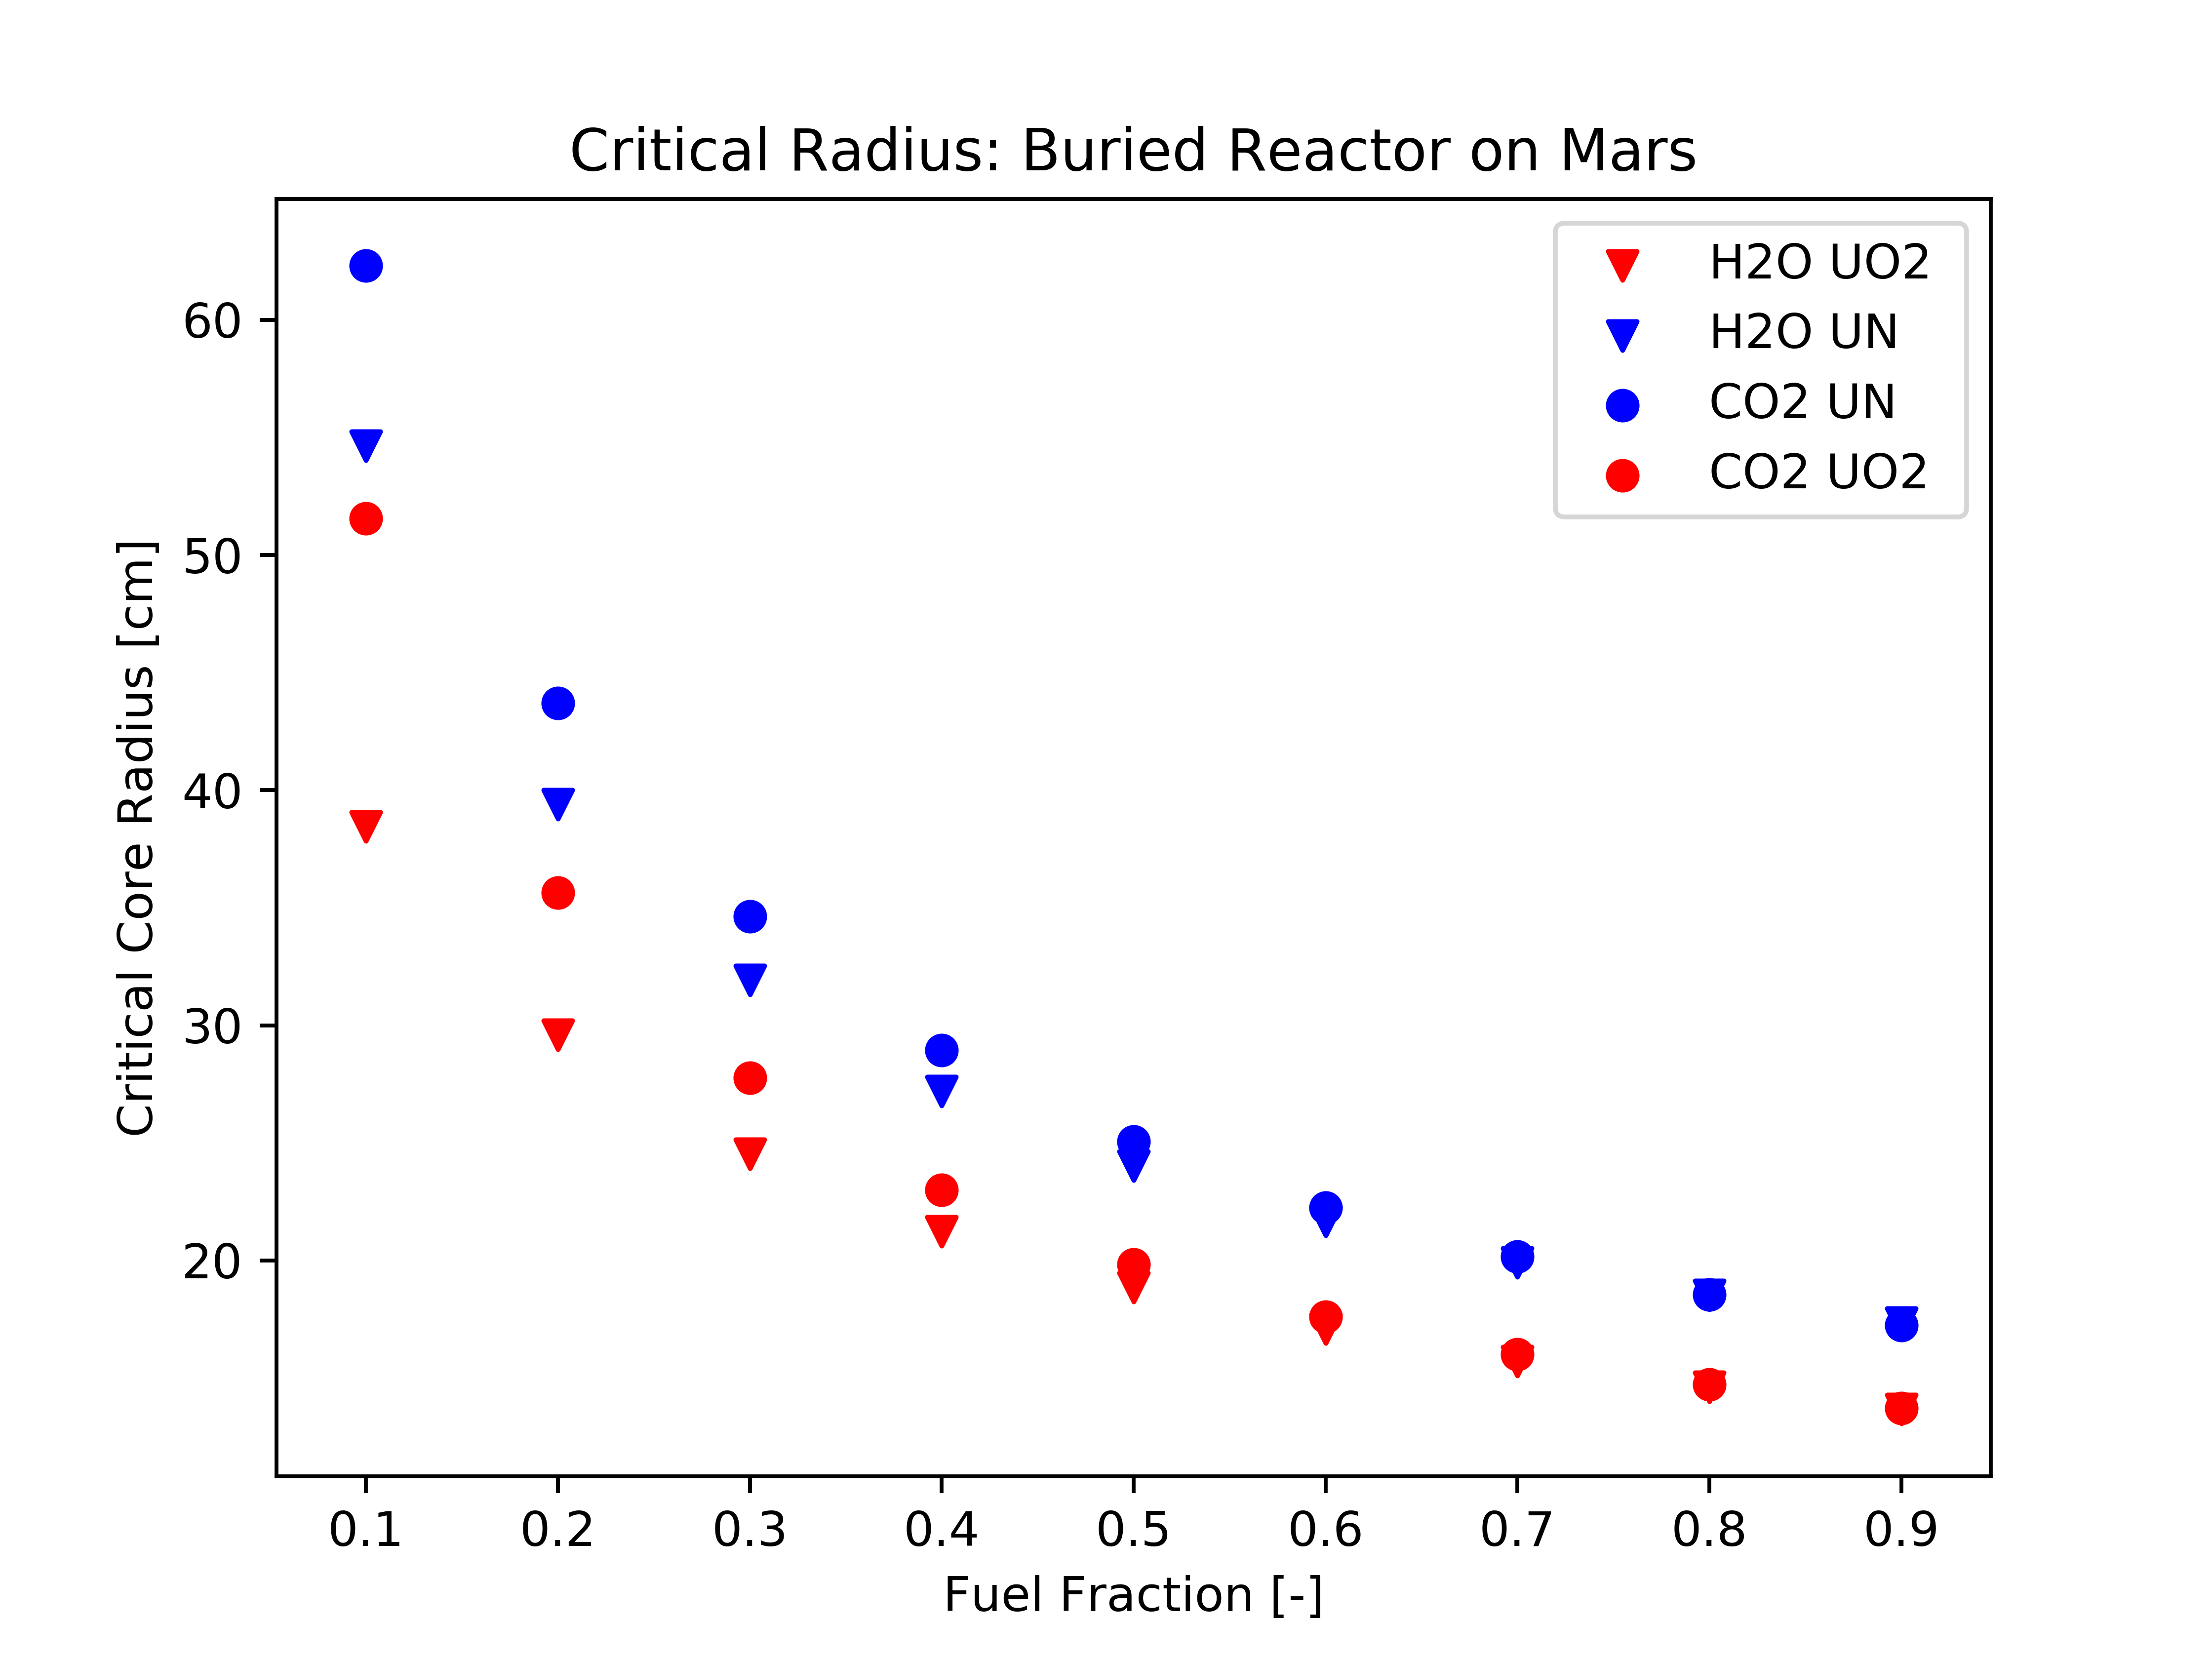
\includegraphics[width=3in]{../images/crit_radius.png}
\caption{Critical core radius results}
\label{fig:crit_core_radius}
\end{figure}

As shown in figure \ref{fig:crit_core_radius}, the \uox fuel outperforms the UW
cermet fuel in terms of critcial mass. This is because of the higher uranium
density in the \uox. The coolants impact critical radius as well. The \water
provides some moderation that helps improve the fission cross section in the
fuel. As the fuel fraction approaches 1, the difference in coolant is
negligible. These results were fit to a power function, shown in Equation
\ref{eq:power_fit}.

\begin{equation}
    R_{core} = A*exp(-B*frac_{fuel})
    \label{eq:power_fit}
\end{equation}

The resulting coefficients for each reactor configuration are shown below in
Table \ref{tab:crit_radius_coeffs}.

\begin{table}[h]
  \centering
  \caption{Critical Radius Fits}
  \begin{tabular}{ccc}
    \toprule
    Reactor Configuration   &   A [cm]  &  B [-]   \\
    \midrule 
     \uox-\codiox	        & 13.224     &  -0.596 \\
     \uox-\water            & 13.674     &  -0.458 \\
     UW-\codiox             & 16.871     &  -0.573 \\
     UW-\water              & 16.817     &  -0.516 \\
  \end{tabular}
  \label{tab:crit_radius_coeffs}
\end{table}
